\section{Render\-GL  Class Reference}
\label{class_RenderGL}\index{RenderGL@{Render\-GL}}
Perform 3D rendering using the GL and GLUT libraries. 


{\tt \#include $<$rendergl.h$>$}

Inheritance diagram for Render\-GL::\begin{figure}[H]
\begin{center}
\leavevmode
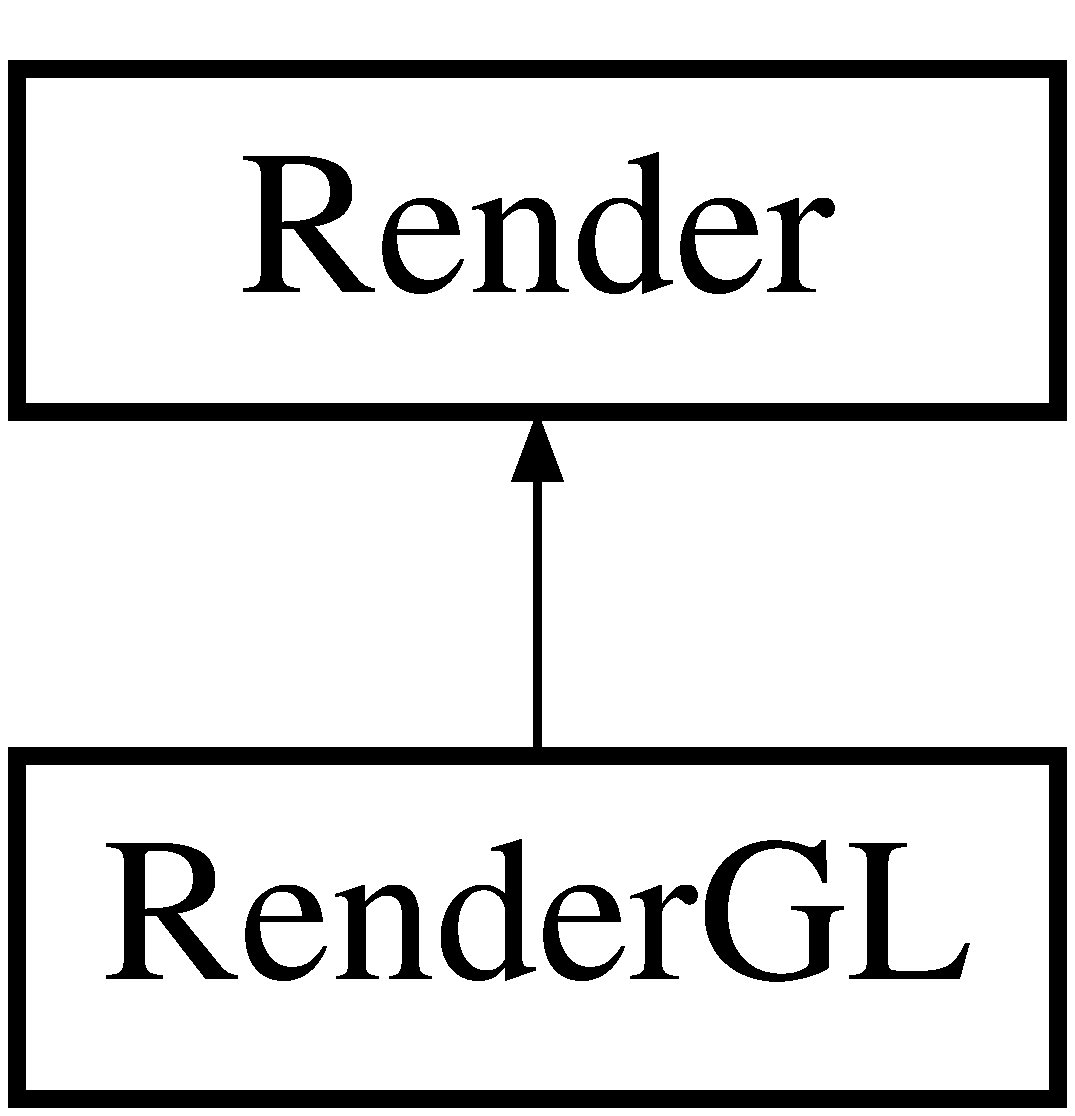
\includegraphics[height=2cm]{class_RenderGL}
\end{center}
\end{figure}
\subsection*{Public Methods}
\begin{CompactItemize}
\item 
{\bf Render\-GL} ()
\item 
{\bf Render\-GL} (string filepath)
\item 
{\bf Render\-GL} ({\bf Scene} $\ast$s, string filepath)
\item 
virtual {\bf $\sim$Render\-GL} ()
\item 
virtual void {\bf Reset} ()
\begin{CompactList}\small\item\em Reset the renderer.\item\end{CompactList}\item 
virtual void {\bf Init} ()
\begin{CompactList}\small\item\em Initialized the renderer.\item\end{CompactList}\item 
virtual void {\bf Main\-Loop} ({\bf Gui} $\ast$g)
\begin{CompactList}\small\item\em If Control\-Freak = true, then Main\-Loop is entered here.\item\end{CompactList}\end{CompactItemize}
\subsection*{Public Attributes}
\begin{CompactItemize}
\item 
{\bf Gui}$\ast$ {\bf G}
\end{CompactItemize}
\subsection*{Static Public Methods}
\begin{CompactItemize}
\item 
void {\bf Glut\-Idle\-Processing} ()
\item 
void {\bf Glut\-Draw\-Environment} ()
\item 
void {\bf Glut\-Reshape} (int w, int h)
\item 
void {\bf Glut\-Mouse} (int button, int state, int x, int y)
\item 
void {\bf Glut\-Mouse\-Move} (int x, int y)
\item 
void {\bf Glut\-Keyboard} (unsigned char Key, int x, int y)
\end{CompactItemize}
\subsection*{Protected Methods}
\begin{CompactItemize}
\item 
void {\bf Load\-Config} ()
\item 
void {\bf Add\-Body\-Object} ({\bf msl\-GLObject} $\ast$obj)
\item 
void {\bf Add\-Env\-Object} ({\bf msl\-GLObject} $\ast$obj)
\item 
{\bf msl\-GLObject}$\ast$ {\bf Which\-Object} (int id)
\item 
void {\bf Scene\-Render} ()
\item 
void {\bf Set\-Light\-Pos} ()
\item 
void {\bf Set\-Scene\-Orientation\-Change} (const {\bf MSLVector} \&oric)
\item 
void {\bf Set\-Scene\-Position\-Change} (const {\bf MSLVector} \&posc)
\item 
void {\bf Set\-Body\-State} (const {\bf MSLVector} \&state)
\item 
void {\bf Set\-Env\-State} (const {\bf MSLVector} \&state)
\item 
void {\bf Draw\-Bounding\-Box} ()
\item 
void {\bf Draw\-Path} ()
\begin{CompactList}\small\item\em Display an entire path (the specific renderer determines how).\item\end{CompactList}\item 
void {\bf Init\-Data} ()
\item 
void {\bf Init\-Geometry} (list$<$ {\bf MSLTriangle} $>$ triangles)
\item 
void {\bf Draw\-Bodies} (const {\bf MSLVector} \&x)
\item 
void {\bf Draw\-Env} ()
\item 
void {\bf Norm\-Cross\-Product} (float v1[3], float v2[3], float out[3])
\item 
void {\bf Normalize} (float v[3])
\item 
void {\bf Show\-Coordinate\-Frame} ()
\end{CompactItemize}
\subsection*{Protected Attributes}
\begin{CompactItemize}
\item 
vector$<$int$>$ {\bf Env\-Index}
\item 
vector$<$int$>$ {\bf Body\-Index}
\item 
float {\bf Window\-X}
\item 
float {\bf Window\-Y}
\item 
float {\bf Window\-Z}
\item 
float {\bf Bounding\-Box\-Min} [3]
\item 
float {\bf Bounding\-Box\-Max} [3]
\item 
float {\bf Orientation} [3]
\item 
float {\bf Position} [3]
\item 
float {\bf Fov}
\item 
float {\bf Aspect\-Ratio}
\item 
float {\bf Near}
\item 
float {\bf Far}
\item 
float {\bf Eye\-X}
\item 
float {\bf Eye\-Y}
\item 
float {\bf Eye\-Z}
\item 
float {\bf Vp\-X}
\item 
float {\bf Vp\-Y}
\item 
float {\bf Vp\-Z}
\item 
float {\bf Vup\-X}
\item 
float {\bf Vup\-Y}
\item 
float {\bf Vup\-Z}
\item 
float {\bf View\-Length}
\item 
{\bf MSLVector} {\bf VCoord\-Z}
\item 
{\bf MSLVector} {\bf VCoord\-Y}
\item 
{\bf MSLVector} {\bf VCoord\-X}
\item 
{\bf MSLVector} {\bf VRpy}
\item 
{\bf MSLVector} {\bf Def\-VCoord\-Z}
\item 
{\bf MSLVector} {\bf Def\-VCoord\-Y}
\item 
{\bf MSLVector} {\bf Def\-VCoord\-X}
\item 
{\bf MSLVector} {\bf Def\-VRpy}
\item 
{\bf MSLVector} {\bf Rpy\-Modification}
\item 
{\bf MSLVector} {\bf SCoord\-Z}
\item 
{\bf MSLVector} {\bf SCoord\-Y}
\item 
{\bf MSLVector} {\bf SCoord\-X}
\item 
float {\bf Light\-Pos\-X}
\item 
float {\bf Light\-Pos\-Y}
\item 
float {\bf Light\-Pos\-Z}
\item 
int {\bf Number\-Of\-Object}
\item 
int {\bf Number\-Of\-Body}
\item 
int {\bf Number\-Of\-Env\-Obj}
\item 
{\bf msl\-GLObject}$\ast$$\ast$ {\bf Scene\-Body\-Lib}
\item 
{\bf msl\-GLObject}$\ast$$\ast$ {\bf Scene\-Env\-Obj\-Lib}
\item 
{\bf MSLVector} {\bf Env\-Transform}
\item 
{\bf MSLVector} {\bf Body\-Transform}
\item 
int {\bf Main\-Window}
\item 
int {\bf Select\-Object\-ID}
\item 
int {\bf Current\-Object}
\item 
int {\bf Current\-Mouse\-Button}
\item 
int {\bf Current\-Mouse\-State}
\item 
int {\bf Current\-Keyboard}
\item 
float {\bf Last\-X}
\item 
float {\bf Last\-Y}
\item 
float {\bf Change\-Rate}
\item 
float {\bf Animation\-Time\-Scale\-Tmp}
\end{CompactItemize}


\subsection{Detailed Description}
Perform 3D rendering using the GL and GLUT libraries.



\subsection{Constructor \& Destructor Documentation}
\index{RenderGL@{Render\-GL}!RenderGL@{RenderGL}}
\index{RenderGL@{RenderGL}!RenderGL@{Render\-GL}}
\subsubsection{\setlength{\rightskip}{0pt plus 5cm}Render\-GL::Render\-GL ()}\label{class_RenderGL_a0}


\index{RenderGL@{Render\-GL}!RenderGL@{RenderGL}}
\index{RenderGL@{RenderGL}!RenderGL@{Render\-GL}}
\subsubsection{\setlength{\rightskip}{0pt plus 5cm}Render\-GL::Render\-GL (string {\em filepath})}\label{class_RenderGL_a1}


\index{RenderGL@{Render\-GL}!RenderGL@{RenderGL}}
\index{RenderGL@{RenderGL}!RenderGL@{Render\-GL}}
\subsubsection{\setlength{\rightskip}{0pt plus 5cm}Render\-GL::Render\-GL ({\bf Scene} $\ast$ {\em s}, string {\em filepath})}\label{class_RenderGL_a2}


\index{RenderGL@{Render\-GL}!~RenderGL@{$\sim$RenderGL}}
\index{~RenderGL@{$\sim$RenderGL}!RenderGL@{Render\-GL}}
\subsubsection{\setlength{\rightskip}{0pt plus 5cm}virtual Render\-GL::$\sim$Render\-GL ()\hspace{0.3cm}{\tt  [virtual]}}\label{class_RenderGL_a3}




\subsection{Member Function Documentation}
\index{RenderGL@{Render\-GL}!AddBodyObject@{AddBodyObject}}
\index{AddBodyObject@{AddBodyObject}!RenderGL@{Render\-GL}}
\subsubsection{\setlength{\rightskip}{0pt plus 5cm}void Render\-GL::Add\-Body\-Object ({\bf msl\-GLObject} $\ast$ {\em obj})\hspace{0.3cm}{\tt  [protected]}}\label{class_RenderGL_b1}


\index{RenderGL@{Render\-GL}!AddEnvObject@{AddEnvObject}}
\index{AddEnvObject@{AddEnvObject}!RenderGL@{Render\-GL}}
\subsubsection{\setlength{\rightskip}{0pt plus 5cm}void Render\-GL::Add\-Env\-Object ({\bf msl\-GLObject} $\ast$ {\em obj})\hspace{0.3cm}{\tt  [protected]}}\label{class_RenderGL_b2}


\index{RenderGL@{Render\-GL}!DrawBodies@{DrawBodies}}
\index{DrawBodies@{DrawBodies}!RenderGL@{Render\-GL}}
\subsubsection{\setlength{\rightskip}{0pt plus 5cm}void Render\-GL::Draw\-Bodies (const {\bf MSLVector} \& {\em x})\hspace{0.3cm}{\tt  [protected]}}\label{class_RenderGL_b14}


\index{RenderGL@{Render\-GL}!DrawBoundingBox@{DrawBoundingBox}}
\index{DrawBoundingBox@{DrawBoundingBox}!RenderGL@{Render\-GL}}
\subsubsection{\setlength{\rightskip}{0pt plus 5cm}void Render\-GL::Draw\-Bounding\-Box ()\hspace{0.3cm}{\tt  [protected]}}\label{class_RenderGL_b10}


\index{RenderGL@{Render\-GL}!DrawEnv@{DrawEnv}}
\index{DrawEnv@{DrawEnv}!RenderGL@{Render\-GL}}
\subsubsection{\setlength{\rightskip}{0pt plus 5cm}void Render\-GL::Draw\-Env ()\hspace{0.3cm}{\tt  [protected]}}\label{class_RenderGL_b15}


\index{RenderGL@{Render\-GL}!DrawPath@{DrawPath}}
\index{DrawPath@{DrawPath}!RenderGL@{Render\-GL}}
\subsubsection{\setlength{\rightskip}{0pt plus 5cm}void Render\-GL::Draw\-Path ()\hspace{0.3cm}{\tt  [protected, virtual]}}\label{class_RenderGL_b11}


Display an entire path (the specific renderer determines how).



Reimplemented from {\bf Render} {\rm (p.\,\pageref{class_Render_a12})}.\index{RenderGL@{Render\-GL}!GlutDrawEnvironment@{GlutDrawEnvironment}}
\index{GlutDrawEnvironment@{GlutDrawEnvironment}!RenderGL@{Render\-GL}}
\subsubsection{\setlength{\rightskip}{0pt plus 5cm}void Render\-GL::Glut\-Draw\-Environment ()\hspace{0.3cm}{\tt  [static]}}\label{class_RenderGL_d1}


\index{RenderGL@{Render\-GL}!GlutIdleProcessing@{GlutIdleProcessing}}
\index{GlutIdleProcessing@{GlutIdleProcessing}!RenderGL@{Render\-GL}}
\subsubsection{\setlength{\rightskip}{0pt plus 5cm}void Render\-GL::Glut\-Idle\-Processing ()\hspace{0.3cm}{\tt  [static]}}\label{class_RenderGL_d0}


\index{RenderGL@{Render\-GL}!GlutKeyboard@{GlutKeyboard}}
\index{GlutKeyboard@{GlutKeyboard}!RenderGL@{Render\-GL}}
\subsubsection{\setlength{\rightskip}{0pt plus 5cm}void Render\-GL::Glut\-Keyboard (unsigned char {\em Key}, int {\em x}, int {\em y})\hspace{0.3cm}{\tt  [static]}}\label{class_RenderGL_d5}


\index{RenderGL@{Render\-GL}!GlutMouse@{GlutMouse}}
\index{GlutMouse@{GlutMouse}!RenderGL@{Render\-GL}}
\subsubsection{\setlength{\rightskip}{0pt plus 5cm}void Render\-GL::Glut\-Mouse (int {\em button}, int {\em state}, int {\em x}, int {\em y})\hspace{0.3cm}{\tt  [static]}}\label{class_RenderGL_d3}


\index{RenderGL@{Render\-GL}!GlutMouseMove@{GlutMouseMove}}
\index{GlutMouseMove@{GlutMouseMove}!RenderGL@{Render\-GL}}
\subsubsection{\setlength{\rightskip}{0pt plus 5cm}void Render\-GL::Glut\-Mouse\-Move (int {\em x}, int {\em y})\hspace{0.3cm}{\tt  [static]}}\label{class_RenderGL_d4}


\index{RenderGL@{Render\-GL}!GlutReshape@{GlutReshape}}
\index{GlutReshape@{GlutReshape}!RenderGL@{Render\-GL}}
\subsubsection{\setlength{\rightskip}{0pt plus 5cm}void Render\-GL::Glut\-Reshape (int {\em w}, int {\em h})\hspace{0.3cm}{\tt  [static]}}\label{class_RenderGL_d2}


\index{RenderGL@{Render\-GL}!Init@{Init}}
\index{Init@{Init}!RenderGL@{Render\-GL}}
\subsubsection{\setlength{\rightskip}{0pt plus 5cm}virtual void Render\-GL::Init ()\hspace{0.3cm}{\tt  [virtual]}}\label{class_RenderGL_a5}


Initialized the renderer.



Reimplemented from {\bf Render} {\rm (p.\,\pageref{class_Render_a4})}.\index{RenderGL@{Render\-GL}!InitData@{InitData}}
\index{InitData@{InitData}!RenderGL@{Render\-GL}}
\subsubsection{\setlength{\rightskip}{0pt plus 5cm}void Render\-GL::Init\-Data ()\hspace{0.3cm}{\tt  [protected]}}\label{class_RenderGL_b12}


\index{RenderGL@{Render\-GL}!InitGeometry@{InitGeometry}}
\index{InitGeometry@{InitGeometry}!RenderGL@{Render\-GL}}
\subsubsection{\setlength{\rightskip}{0pt plus 5cm}void Render\-GL::Init\-Geometry (list$<$ {\bf MSLTriangle} $>$ {\em triangles})\hspace{0.3cm}{\tt  [protected]}}\label{class_RenderGL_b13}


\index{RenderGL@{Render\-GL}!LoadConfig@{LoadConfig}}
\index{LoadConfig@{LoadConfig}!RenderGL@{Render\-GL}}
\subsubsection{\setlength{\rightskip}{0pt plus 5cm}void Render\-GL::Load\-Config ()\hspace{0.3cm}{\tt  [protected]}}\label{class_RenderGL_b0}


\index{RenderGL@{Render\-GL}!MainLoop@{MainLoop}}
\index{MainLoop@{MainLoop}!RenderGL@{Render\-GL}}
\subsubsection{\setlength{\rightskip}{0pt plus 5cm}virtual void Render\-GL::Main\-Loop ({\bf Gui} $\ast$ {\em g})\hspace{0.3cm}{\tt  [virtual]}}\label{class_RenderGL_a6}


If Control\-Freak = true, then Main\-Loop is entered here.



Reimplemented from {\bf Render} {\rm (p.\,\pageref{class_Render_a6})}.\index{RenderGL@{Render\-GL}!NormCrossProduct@{NormCrossProduct}}
\index{NormCrossProduct@{NormCrossProduct}!RenderGL@{Render\-GL}}
\subsubsection{\setlength{\rightskip}{0pt plus 5cm}void Render\-GL::Norm\-Cross\-Product (float {\em v1}[3], float {\em v2}[3], float {\em out}[3])\hspace{0.3cm}{\tt  [protected]}}\label{class_RenderGL_b16}


\index{RenderGL@{Render\-GL}!Normalize@{Normalize}}
\index{Normalize@{Normalize}!RenderGL@{Render\-GL}}
\subsubsection{\setlength{\rightskip}{0pt plus 5cm}void Render\-GL::Normalize (float {\em v}[3])\hspace{0.3cm}{\tt  [protected]}}\label{class_RenderGL_b17}


\index{RenderGL@{Render\-GL}!Reset@{Reset}}
\index{Reset@{Reset}!RenderGL@{Render\-GL}}
\subsubsection{\setlength{\rightskip}{0pt plus 5cm}virtual void Render\-GL::Reset ()\hspace{0.3cm}{\tt  [virtual]}}\label{class_RenderGL_a4}


Reset the renderer.



Reimplemented from {\bf Render} {\rm (p.\,\pageref{class_Render_a7})}.\index{RenderGL@{Render\-GL}!SceneRender@{SceneRender}}
\index{SceneRender@{SceneRender}!RenderGL@{Render\-GL}}
\subsubsection{\setlength{\rightskip}{0pt plus 5cm}void Render\-GL::Scene\-Render ()\hspace{0.3cm}{\tt  [protected]}}\label{class_RenderGL_b4}


\index{RenderGL@{Render\-GL}!SetBodyState@{SetBodyState}}
\index{SetBodyState@{SetBodyState}!RenderGL@{Render\-GL}}
\subsubsection{\setlength{\rightskip}{0pt plus 5cm}void Render\-GL::Set\-Body\-State (const {\bf MSLVector} \& {\em state})\hspace{0.3cm}{\tt  [protected]}}\label{class_RenderGL_b8}


\index{RenderGL@{Render\-GL}!SetEnvState@{SetEnvState}}
\index{SetEnvState@{SetEnvState}!RenderGL@{Render\-GL}}
\subsubsection{\setlength{\rightskip}{0pt plus 5cm}void Render\-GL::Set\-Env\-State (const {\bf MSLVector} \& {\em state})\hspace{0.3cm}{\tt  [protected]}}\label{class_RenderGL_b9}


\index{RenderGL@{Render\-GL}!SetLightPos@{SetLightPos}}
\index{SetLightPos@{SetLightPos}!RenderGL@{Render\-GL}}
\subsubsection{\setlength{\rightskip}{0pt plus 5cm}void Render\-GL::Set\-Light\-Pos ()\hspace{0.3cm}{\tt  [protected]}}\label{class_RenderGL_b5}


\index{RenderGL@{Render\-GL}!SetSceneOrientationChange@{SetSceneOrientationChange}}
\index{SetSceneOrientationChange@{SetSceneOrientationChange}!RenderGL@{Render\-GL}}
\subsubsection{\setlength{\rightskip}{0pt plus 5cm}void Render\-GL::Set\-Scene\-Orientation\-Change (const {\bf MSLVector} \& {\em oric})\hspace{0.3cm}{\tt  [protected]}}\label{class_RenderGL_b6}


\index{RenderGL@{Render\-GL}!SetScenePositionChange@{SetScenePositionChange}}
\index{SetScenePositionChange@{SetScenePositionChange}!RenderGL@{Render\-GL}}
\subsubsection{\setlength{\rightskip}{0pt plus 5cm}void Render\-GL::Set\-Scene\-Position\-Change (const {\bf MSLVector} \& {\em posc})\hspace{0.3cm}{\tt  [protected]}}\label{class_RenderGL_b7}


\index{RenderGL@{Render\-GL}!ShowCoordinateFrame@{ShowCoordinateFrame}}
\index{ShowCoordinateFrame@{ShowCoordinateFrame}!RenderGL@{Render\-GL}}
\subsubsection{\setlength{\rightskip}{0pt plus 5cm}void Render\-GL::Show\-Coordinate\-Frame ()\hspace{0.3cm}{\tt  [protected]}}\label{class_RenderGL_b18}


\index{RenderGL@{Render\-GL}!WhichObject@{WhichObject}}
\index{WhichObject@{WhichObject}!RenderGL@{Render\-GL}}
\subsubsection{\setlength{\rightskip}{0pt plus 5cm}{\bf msl\-GLObject}$\ast$ Render\-GL::Which\-Object (int {\em id})\hspace{0.3cm}{\tt  [protected]}}\label{class_RenderGL_b3}




\subsection{Member Data Documentation}
\index{RenderGL@{Render\-GL}!AnimationTimeScaleTmp@{AnimationTimeScaleTmp}}
\index{AnimationTimeScaleTmp@{AnimationTimeScaleTmp}!RenderGL@{Render\-GL}}
\subsubsection{\setlength{\rightskip}{0pt plus 5cm}float Render\-GL::Animation\-Time\-Scale\-Tmp\hspace{0.3cm}{\tt  [protected]}}\label{class_RenderGL_n54}


\index{RenderGL@{Render\-GL}!AspectRatio@{AspectRatio}}
\index{AspectRatio@{AspectRatio}!RenderGL@{Render\-GL}}
\subsubsection{\setlength{\rightskip}{0pt plus 5cm}float Render\-GL::Aspect\-Ratio\hspace{0.3cm}{\tt  [protected]}}\label{class_RenderGL_n10}


\index{RenderGL@{Render\-GL}!BodyIndex@{BodyIndex}}
\index{BodyIndex@{BodyIndex}!RenderGL@{Render\-GL}}
\subsubsection{\setlength{\rightskip}{0pt plus 5cm}vector$<$int$>$ Render\-GL::Body\-Index\hspace{0.3cm}{\tt  [protected]}}\label{class_RenderGL_n1}


\index{RenderGL@{Render\-GL}!BodyTransform@{BodyTransform}}
\index{BodyTransform@{BodyTransform}!RenderGL@{Render\-GL}}
\subsubsection{\setlength{\rightskip}{0pt plus 5cm}{\bf MSLVector} Render\-GL::Body\-Transform\hspace{0.3cm}{\tt  [protected]}}\label{class_RenderGL_n44}


\index{RenderGL@{Render\-GL}!BoundingBoxMax@{BoundingBoxMax}}
\index{BoundingBoxMax@{BoundingBoxMax}!RenderGL@{Render\-GL}}
\subsubsection{\setlength{\rightskip}{0pt plus 5cm}float Render\-GL::Bounding\-Box\-Max[3]\hspace{0.3cm}{\tt  [protected]}}\label{class_RenderGL_n6}


\index{RenderGL@{Render\-GL}!BoundingBoxMin@{BoundingBoxMin}}
\index{BoundingBoxMin@{BoundingBoxMin}!RenderGL@{Render\-GL}}
\subsubsection{\setlength{\rightskip}{0pt plus 5cm}float Render\-GL::Bounding\-Box\-Min[3]\hspace{0.3cm}{\tt  [protected]}}\label{class_RenderGL_n5}


\index{RenderGL@{Render\-GL}!ChangeRate@{ChangeRate}}
\index{ChangeRate@{ChangeRate}!RenderGL@{Render\-GL}}
\subsubsection{\setlength{\rightskip}{0pt plus 5cm}float Render\-GL::Change\-Rate\hspace{0.3cm}{\tt  [protected]}}\label{class_RenderGL_n53}


\index{RenderGL@{Render\-GL}!CurrentKeyboard@{CurrentKeyboard}}
\index{CurrentKeyboard@{CurrentKeyboard}!RenderGL@{Render\-GL}}
\subsubsection{\setlength{\rightskip}{0pt plus 5cm}int Render\-GL::Current\-Keyboard\hspace{0.3cm}{\tt  [protected]}}\label{class_RenderGL_n50}


\index{RenderGL@{Render\-GL}!CurrentMouseButton@{CurrentMouseButton}}
\index{CurrentMouseButton@{CurrentMouseButton}!RenderGL@{Render\-GL}}
\subsubsection{\setlength{\rightskip}{0pt plus 5cm}int Render\-GL::Current\-Mouse\-Button\hspace{0.3cm}{\tt  [protected]}}\label{class_RenderGL_n48}


\index{RenderGL@{Render\-GL}!CurrentMouseState@{CurrentMouseState}}
\index{CurrentMouseState@{CurrentMouseState}!RenderGL@{Render\-GL}}
\subsubsection{\setlength{\rightskip}{0pt plus 5cm}int Render\-GL::Current\-Mouse\-State\hspace{0.3cm}{\tt  [protected]}}\label{class_RenderGL_n49}


\index{RenderGL@{Render\-GL}!CurrentObject@{CurrentObject}}
\index{CurrentObject@{CurrentObject}!RenderGL@{Render\-GL}}
\subsubsection{\setlength{\rightskip}{0pt plus 5cm}int Render\-GL::Current\-Object\hspace{0.3cm}{\tt  [protected]}}\label{class_RenderGL_n47}


\index{RenderGL@{Render\-GL}!DefVCoordX@{DefVCoordX}}
\index{DefVCoordX@{DefVCoordX}!RenderGL@{Render\-GL}}
\subsubsection{\setlength{\rightskip}{0pt plus 5cm}{\bf MSLVector} Render\-GL::Def\-VCoord\-X\hspace{0.3cm}{\tt  [protected]}}\label{class_RenderGL_n29}


\index{RenderGL@{Render\-GL}!DefVCoordY@{DefVCoordY}}
\index{DefVCoordY@{DefVCoordY}!RenderGL@{Render\-GL}}
\subsubsection{\setlength{\rightskip}{0pt plus 5cm}{\bf MSLVector} Render\-GL::Def\-VCoord\-Y\hspace{0.3cm}{\tt  [protected]}}\label{class_RenderGL_n28}


\index{RenderGL@{Render\-GL}!DefVCoordZ@{DefVCoordZ}}
\index{DefVCoordZ@{DefVCoordZ}!RenderGL@{Render\-GL}}
\subsubsection{\setlength{\rightskip}{0pt plus 5cm}{\bf MSLVector} Render\-GL::Def\-VCoord\-Z\hspace{0.3cm}{\tt  [protected]}}\label{class_RenderGL_n27}


\index{RenderGL@{Render\-GL}!DefVRpy@{DefVRpy}}
\index{DefVRpy@{DefVRpy}!RenderGL@{Render\-GL}}
\subsubsection{\setlength{\rightskip}{0pt plus 5cm}{\bf MSLVector} Render\-GL::Def\-VRpy\hspace{0.3cm}{\tt  [protected]}}\label{class_RenderGL_n30}


\index{RenderGL@{Render\-GL}!EnvIndex@{EnvIndex}}
\index{EnvIndex@{EnvIndex}!RenderGL@{Render\-GL}}
\subsubsection{\setlength{\rightskip}{0pt plus 5cm}vector$<$int$>$ Render\-GL::Env\-Index\hspace{0.3cm}{\tt  [protected]}}\label{class_RenderGL_n0}


\index{RenderGL@{Render\-GL}!EnvTransform@{EnvTransform}}
\index{EnvTransform@{EnvTransform}!RenderGL@{Render\-GL}}
\subsubsection{\setlength{\rightskip}{0pt plus 5cm}{\bf MSLVector} Render\-GL::Env\-Transform\hspace{0.3cm}{\tt  [protected]}}\label{class_RenderGL_n43}


\index{RenderGL@{Render\-GL}!EyeX@{EyeX}}
\index{EyeX@{EyeX}!RenderGL@{Render\-GL}}
\subsubsection{\setlength{\rightskip}{0pt plus 5cm}float Render\-GL::Eye\-X\hspace{0.3cm}{\tt  [protected]}}\label{class_RenderGL_n13}


\index{RenderGL@{Render\-GL}!EyeY@{EyeY}}
\index{EyeY@{EyeY}!RenderGL@{Render\-GL}}
\subsubsection{\setlength{\rightskip}{0pt plus 5cm}float Render\-GL::Eye\-Y\hspace{0.3cm}{\tt  [protected]}}\label{class_RenderGL_n14}


\index{RenderGL@{Render\-GL}!EyeZ@{EyeZ}}
\index{EyeZ@{EyeZ}!RenderGL@{Render\-GL}}
\subsubsection{\setlength{\rightskip}{0pt plus 5cm}float Render\-GL::Eye\-Z\hspace{0.3cm}{\tt  [protected]}}\label{class_RenderGL_n15}


\index{RenderGL@{Render\-GL}!Far@{Far}}
\index{Far@{Far}!RenderGL@{Render\-GL}}
\subsubsection{\setlength{\rightskip}{0pt plus 5cm}float Render\-GL::Far\hspace{0.3cm}{\tt  [protected]}}\label{class_RenderGL_n12}


\index{RenderGL@{Render\-GL}!Fov@{Fov}}
\index{Fov@{Fov}!RenderGL@{Render\-GL}}
\subsubsection{\setlength{\rightskip}{0pt plus 5cm}float Render\-GL::Fov\hspace{0.3cm}{\tt  [protected]}}\label{class_RenderGL_n9}


\index{RenderGL@{Render\-GL}!G@{G}}
\index{G@{G}!RenderGL@{Render\-GL}}
\subsubsection{\setlength{\rightskip}{0pt plus 5cm}{\bf Gui}$\ast$ Render\-GL::G}\label{class_RenderGL_m0}


\index{RenderGL@{Render\-GL}!LastX@{LastX}}
\index{LastX@{LastX}!RenderGL@{Render\-GL}}
\subsubsection{\setlength{\rightskip}{0pt plus 5cm}float Render\-GL::Last\-X\hspace{0.3cm}{\tt  [protected]}}\label{class_RenderGL_n51}


\index{RenderGL@{Render\-GL}!LastY@{LastY}}
\index{LastY@{LastY}!RenderGL@{Render\-GL}}
\subsubsection{\setlength{\rightskip}{0pt plus 5cm}float Render\-GL::Last\-Y\hspace{0.3cm}{\tt  [protected]}}\label{class_RenderGL_n52}


\index{RenderGL@{Render\-GL}!LightPosX@{LightPosX}}
\index{LightPosX@{LightPosX}!RenderGL@{Render\-GL}}
\subsubsection{\setlength{\rightskip}{0pt plus 5cm}float Render\-GL::Light\-Pos\-X\hspace{0.3cm}{\tt  [protected]}}\label{class_RenderGL_n35}


\index{RenderGL@{Render\-GL}!LightPosY@{LightPosY}}
\index{LightPosY@{LightPosY}!RenderGL@{Render\-GL}}
\subsubsection{\setlength{\rightskip}{0pt plus 5cm}float Render\-GL::Light\-Pos\-Y\hspace{0.3cm}{\tt  [protected]}}\label{class_RenderGL_n36}


\index{RenderGL@{Render\-GL}!LightPosZ@{LightPosZ}}
\index{LightPosZ@{LightPosZ}!RenderGL@{Render\-GL}}
\subsubsection{\setlength{\rightskip}{0pt plus 5cm}float Render\-GL::Light\-Pos\-Z\hspace{0.3cm}{\tt  [protected]}}\label{class_RenderGL_n37}


\index{RenderGL@{Render\-GL}!MainWindow@{MainWindow}}
\index{MainWindow@{MainWindow}!RenderGL@{Render\-GL}}
\subsubsection{\setlength{\rightskip}{0pt plus 5cm}int Render\-GL::Main\-Window\hspace{0.3cm}{\tt  [protected]}}\label{class_RenderGL_n45}


\index{RenderGL@{Render\-GL}!Near@{Near}}
\index{Near@{Near}!RenderGL@{Render\-GL}}
\subsubsection{\setlength{\rightskip}{0pt plus 5cm}float Render\-GL::Near\hspace{0.3cm}{\tt  [protected]}}\label{class_RenderGL_n11}


\index{RenderGL@{Render\-GL}!NumberOfBody@{NumberOfBody}}
\index{NumberOfBody@{NumberOfBody}!RenderGL@{Render\-GL}}
\subsubsection{\setlength{\rightskip}{0pt plus 5cm}int Render\-GL::Number\-Of\-Body\hspace{0.3cm}{\tt  [protected]}}\label{class_RenderGL_n39}


\index{RenderGL@{Render\-GL}!NumberOfEnvObj@{NumberOfEnvObj}}
\index{NumberOfEnvObj@{NumberOfEnvObj}!RenderGL@{Render\-GL}}
\subsubsection{\setlength{\rightskip}{0pt plus 5cm}int Render\-GL::Number\-Of\-Env\-Obj\hspace{0.3cm}{\tt  [protected]}}\label{class_RenderGL_n40}


\index{RenderGL@{Render\-GL}!NumberOfObject@{NumberOfObject}}
\index{NumberOfObject@{NumberOfObject}!RenderGL@{Render\-GL}}
\subsubsection{\setlength{\rightskip}{0pt plus 5cm}int Render\-GL::Number\-Of\-Object\hspace{0.3cm}{\tt  [protected]}}\label{class_RenderGL_n38}


\index{RenderGL@{Render\-GL}!Orientation@{Orientation}}
\index{Orientation@{Orientation}!RenderGL@{Render\-GL}}
\subsubsection{\setlength{\rightskip}{0pt plus 5cm}float Render\-GL::Orientation[3]\hspace{0.3cm}{\tt  [protected]}}\label{class_RenderGL_n7}


\index{RenderGL@{Render\-GL}!Position@{Position}}
\index{Position@{Position}!RenderGL@{Render\-GL}}
\subsubsection{\setlength{\rightskip}{0pt plus 5cm}float Render\-GL::Position[3]\hspace{0.3cm}{\tt  [protected]}}\label{class_RenderGL_n8}


\index{RenderGL@{Render\-GL}!RpyModification@{RpyModification}}
\index{RpyModification@{RpyModification}!RenderGL@{Render\-GL}}
\subsubsection{\setlength{\rightskip}{0pt plus 5cm}{\bf MSLVector} Render\-GL::Rpy\-Modification\hspace{0.3cm}{\tt  [protected]}}\label{class_RenderGL_n31}


\index{RenderGL@{Render\-GL}!SCoordX@{SCoordX}}
\index{SCoordX@{SCoordX}!RenderGL@{Render\-GL}}
\subsubsection{\setlength{\rightskip}{0pt plus 5cm}{\bf MSLVector} Render\-GL::SCoord\-X\hspace{0.3cm}{\tt  [protected]}}\label{class_RenderGL_n34}


\index{RenderGL@{Render\-GL}!SCoordY@{SCoordY}}
\index{SCoordY@{SCoordY}!RenderGL@{Render\-GL}}
\subsubsection{\setlength{\rightskip}{0pt plus 5cm}{\bf MSLVector} Render\-GL::SCoord\-Y\hspace{0.3cm}{\tt  [protected]}}\label{class_RenderGL_n33}


\index{RenderGL@{Render\-GL}!SCoordZ@{SCoordZ}}
\index{SCoordZ@{SCoordZ}!RenderGL@{Render\-GL}}
\subsubsection{\setlength{\rightskip}{0pt plus 5cm}{\bf MSLVector} Render\-GL::SCoord\-Z\hspace{0.3cm}{\tt  [protected]}}\label{class_RenderGL_n32}


\index{RenderGL@{Render\-GL}!SceneBodyLib@{SceneBodyLib}}
\index{SceneBodyLib@{SceneBodyLib}!RenderGL@{Render\-GL}}
\subsubsection{\setlength{\rightskip}{0pt plus 5cm}{\bf msl\-GLObject}$\ast$$\ast$ Render\-GL::Scene\-Body\-Lib\hspace{0.3cm}{\tt  [protected]}}\label{class_RenderGL_n41}


\index{RenderGL@{Render\-GL}!SceneEnvObjLib@{SceneEnvObjLib}}
\index{SceneEnvObjLib@{SceneEnvObjLib}!RenderGL@{Render\-GL}}
\subsubsection{\setlength{\rightskip}{0pt plus 5cm}{\bf msl\-GLObject}$\ast$$\ast$ Render\-GL::Scene\-Env\-Obj\-Lib\hspace{0.3cm}{\tt  [protected]}}\label{class_RenderGL_n42}


\index{RenderGL@{Render\-GL}!SelectObjectID@{SelectObjectID}}
\index{SelectObjectID@{SelectObjectID}!RenderGL@{Render\-GL}}
\subsubsection{\setlength{\rightskip}{0pt plus 5cm}int Render\-GL::Select\-Object\-ID\hspace{0.3cm}{\tt  [protected]}}\label{class_RenderGL_n46}


\index{RenderGL@{Render\-GL}!VCoordX@{VCoordX}}
\index{VCoordX@{VCoordX}!RenderGL@{Render\-GL}}
\subsubsection{\setlength{\rightskip}{0pt plus 5cm}{\bf MSLVector} Render\-GL::VCoord\-X\hspace{0.3cm}{\tt  [protected]}}\label{class_RenderGL_n25}


\index{RenderGL@{Render\-GL}!VCoordY@{VCoordY}}
\index{VCoordY@{VCoordY}!RenderGL@{Render\-GL}}
\subsubsection{\setlength{\rightskip}{0pt plus 5cm}{\bf MSLVector} Render\-GL::VCoord\-Y\hspace{0.3cm}{\tt  [protected]}}\label{class_RenderGL_n24}


\index{RenderGL@{Render\-GL}!VCoordZ@{VCoordZ}}
\index{VCoordZ@{VCoordZ}!RenderGL@{Render\-GL}}
\subsubsection{\setlength{\rightskip}{0pt plus 5cm}{\bf MSLVector} Render\-GL::VCoord\-Z\hspace{0.3cm}{\tt  [protected]}}\label{class_RenderGL_n23}


\index{RenderGL@{Render\-GL}!VRpy@{VRpy}}
\index{VRpy@{VRpy}!RenderGL@{Render\-GL}}
\subsubsection{\setlength{\rightskip}{0pt plus 5cm}{\bf MSLVector} Render\-GL::VRpy\hspace{0.3cm}{\tt  [protected]}}\label{class_RenderGL_n26}


\index{RenderGL@{Render\-GL}!ViewLength@{ViewLength}}
\index{ViewLength@{ViewLength}!RenderGL@{Render\-GL}}
\subsubsection{\setlength{\rightskip}{0pt plus 5cm}float Render\-GL::View\-Length\hspace{0.3cm}{\tt  [protected]}}\label{class_RenderGL_n22}


\index{RenderGL@{Render\-GL}!VpX@{VpX}}
\index{VpX@{VpX}!RenderGL@{Render\-GL}}
\subsubsection{\setlength{\rightskip}{0pt plus 5cm}float Render\-GL::Vp\-X\hspace{0.3cm}{\tt  [protected]}}\label{class_RenderGL_n16}


\index{RenderGL@{Render\-GL}!VpY@{VpY}}
\index{VpY@{VpY}!RenderGL@{Render\-GL}}
\subsubsection{\setlength{\rightskip}{0pt plus 5cm}float Render\-GL::Vp\-Y\hspace{0.3cm}{\tt  [protected]}}\label{class_RenderGL_n17}


\index{RenderGL@{Render\-GL}!VpZ@{VpZ}}
\index{VpZ@{VpZ}!RenderGL@{Render\-GL}}
\subsubsection{\setlength{\rightskip}{0pt plus 5cm}float Render\-GL::Vp\-Z\hspace{0.3cm}{\tt  [protected]}}\label{class_RenderGL_n18}


\index{RenderGL@{Render\-GL}!VupX@{VupX}}
\index{VupX@{VupX}!RenderGL@{Render\-GL}}
\subsubsection{\setlength{\rightskip}{0pt plus 5cm}float Render\-GL::Vup\-X\hspace{0.3cm}{\tt  [protected]}}\label{class_RenderGL_n19}


\index{RenderGL@{Render\-GL}!VupY@{VupY}}
\index{VupY@{VupY}!RenderGL@{Render\-GL}}
\subsubsection{\setlength{\rightskip}{0pt plus 5cm}float Render\-GL::Vup\-Y\hspace{0.3cm}{\tt  [protected]}}\label{class_RenderGL_n20}


\index{RenderGL@{Render\-GL}!VupZ@{VupZ}}
\index{VupZ@{VupZ}!RenderGL@{Render\-GL}}
\subsubsection{\setlength{\rightskip}{0pt plus 5cm}float Render\-GL::Vup\-Z\hspace{0.3cm}{\tt  [protected]}}\label{class_RenderGL_n21}


\index{RenderGL@{Render\-GL}!WindowX@{WindowX}}
\index{WindowX@{WindowX}!RenderGL@{Render\-GL}}
\subsubsection{\setlength{\rightskip}{0pt plus 5cm}float Render\-GL::Window\-X\hspace{0.3cm}{\tt  [protected]}}\label{class_RenderGL_n2}


\index{RenderGL@{Render\-GL}!WindowY@{WindowY}}
\index{WindowY@{WindowY}!RenderGL@{Render\-GL}}
\subsubsection{\setlength{\rightskip}{0pt plus 5cm}float Render\-GL::Window\-Y\hspace{0.3cm}{\tt  [protected]}}\label{class_RenderGL_n3}


\index{RenderGL@{Render\-GL}!WindowZ@{WindowZ}}
\index{WindowZ@{WindowZ}!RenderGL@{Render\-GL}}
\subsubsection{\setlength{\rightskip}{0pt plus 5cm}float Render\-GL::Window\-Z\hspace{0.3cm}{\tt  [protected]}}\label{class_RenderGL_n4}




The documentation for this class was generated from the following file:\begin{CompactItemize}
\item 
{\bf rendergl.h}\end{CompactItemize}
